\chapter{Batteries}
To operate the car is required two main source of power coming from two distinct sets of batteries. The main battery is an high voltage \gls{DC} pack. To activate it is necessary a 24V source. For that is required a secondary power source, where it is extracted the low voltage.
They contain a \gls{BMS} managed by a micro controller with whom the user interacts to activate the high voltage section and get information about the status of battery. The communication is performed via CAN interface.

Currently is used two independent set of batteries to provide low voltage. A pack with 24V and another with 12V. However is currently in study and design a single pack with 48V  of nominal voltage with integrated \gls{BMS} to unify the low voltage source and intermediate \gls{DC}-\gls{DC} switching converters will be used to provide 24V and 12V rails.

The low voltage sources are enabled via an emergency button, located near the handbrake (see figure \ref{fig:emergency_button}). In case of any emergency, hit this button and power is cut to the main battery battery pack, causing the vehicle to be on free wheel.

\begin{figure}[!h]
	\centering
	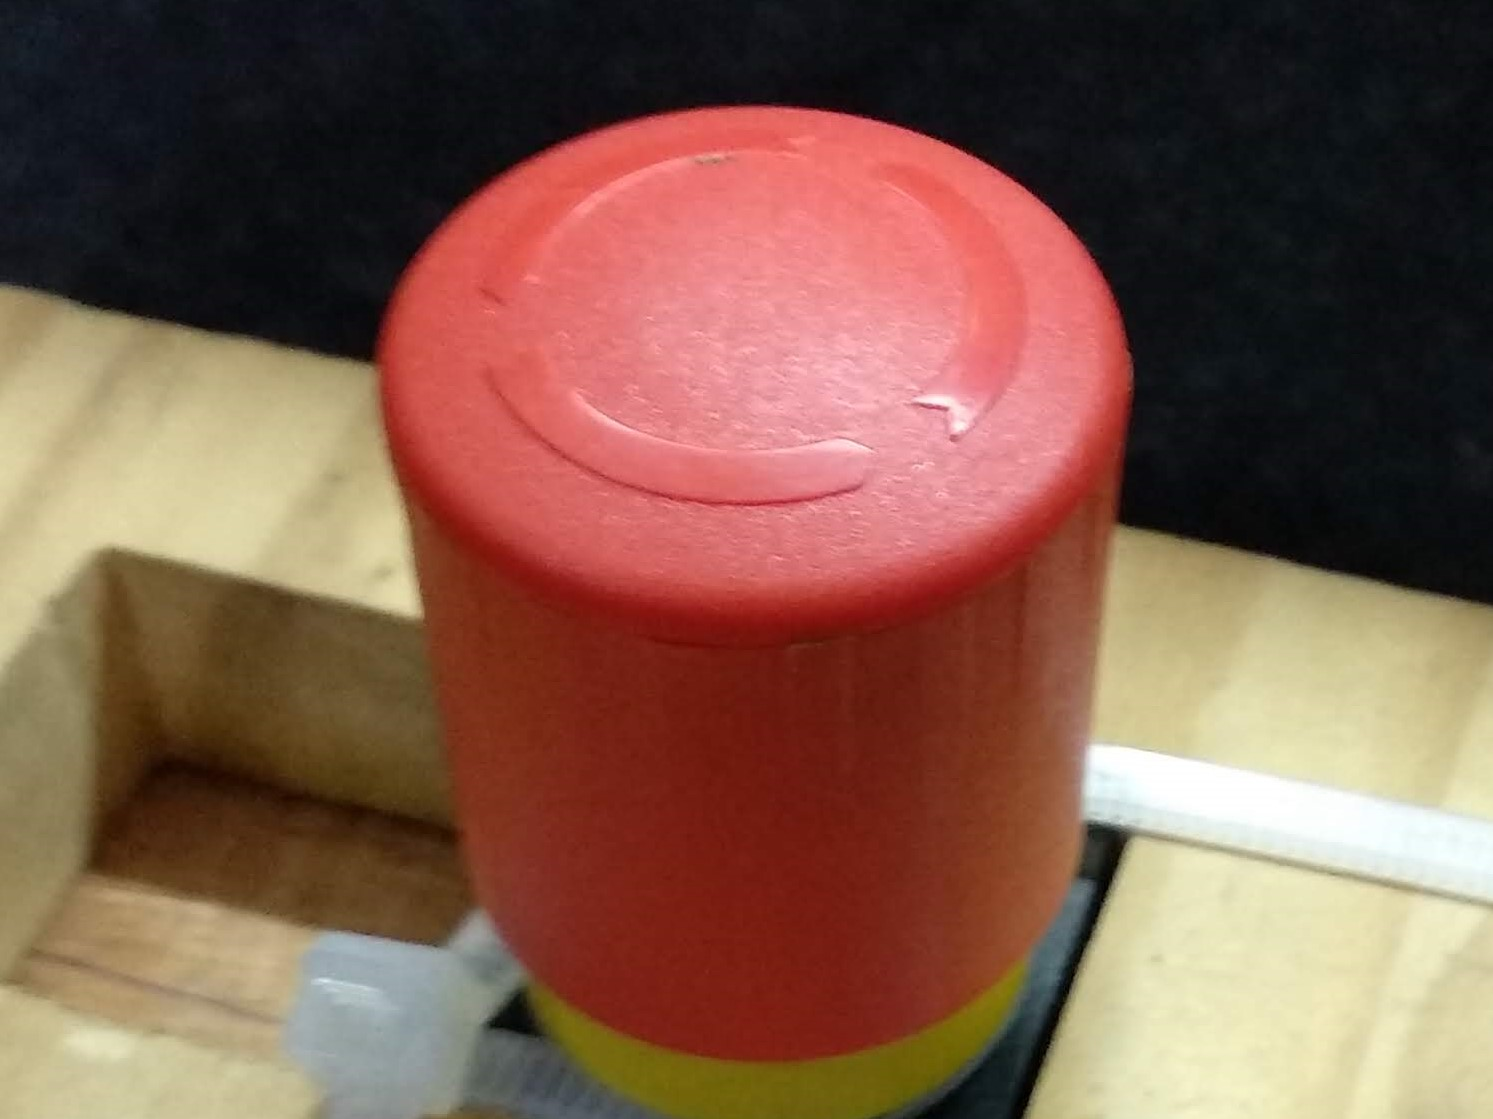
\includegraphics[width=0.4\linewidth]{figures/emergency_button}
	\caption{Emergency button}
	\label{fig:emergency_button}
\end{figure}

\section{Main battery packs}
The power train battery consists in two interconnected battery packs each other with 72 individual cells arranged inside in groups of 12 cells. Both pack are connected in series deploying the total voltage for the Siemens power inverter. The battery pack specifications are present in table \ref{tab:battery_pack_specs}. The main battery connections are shown in figure \ref{fig:battery_connections} In orange is seen the high voltage connectors and the black ones are the low voltage and also control system connectors. Internally, each pack contains a master controller and six controller slaves associated to each of the twelve cells individual groups.

\begin{figure}[!h]
	\centering
	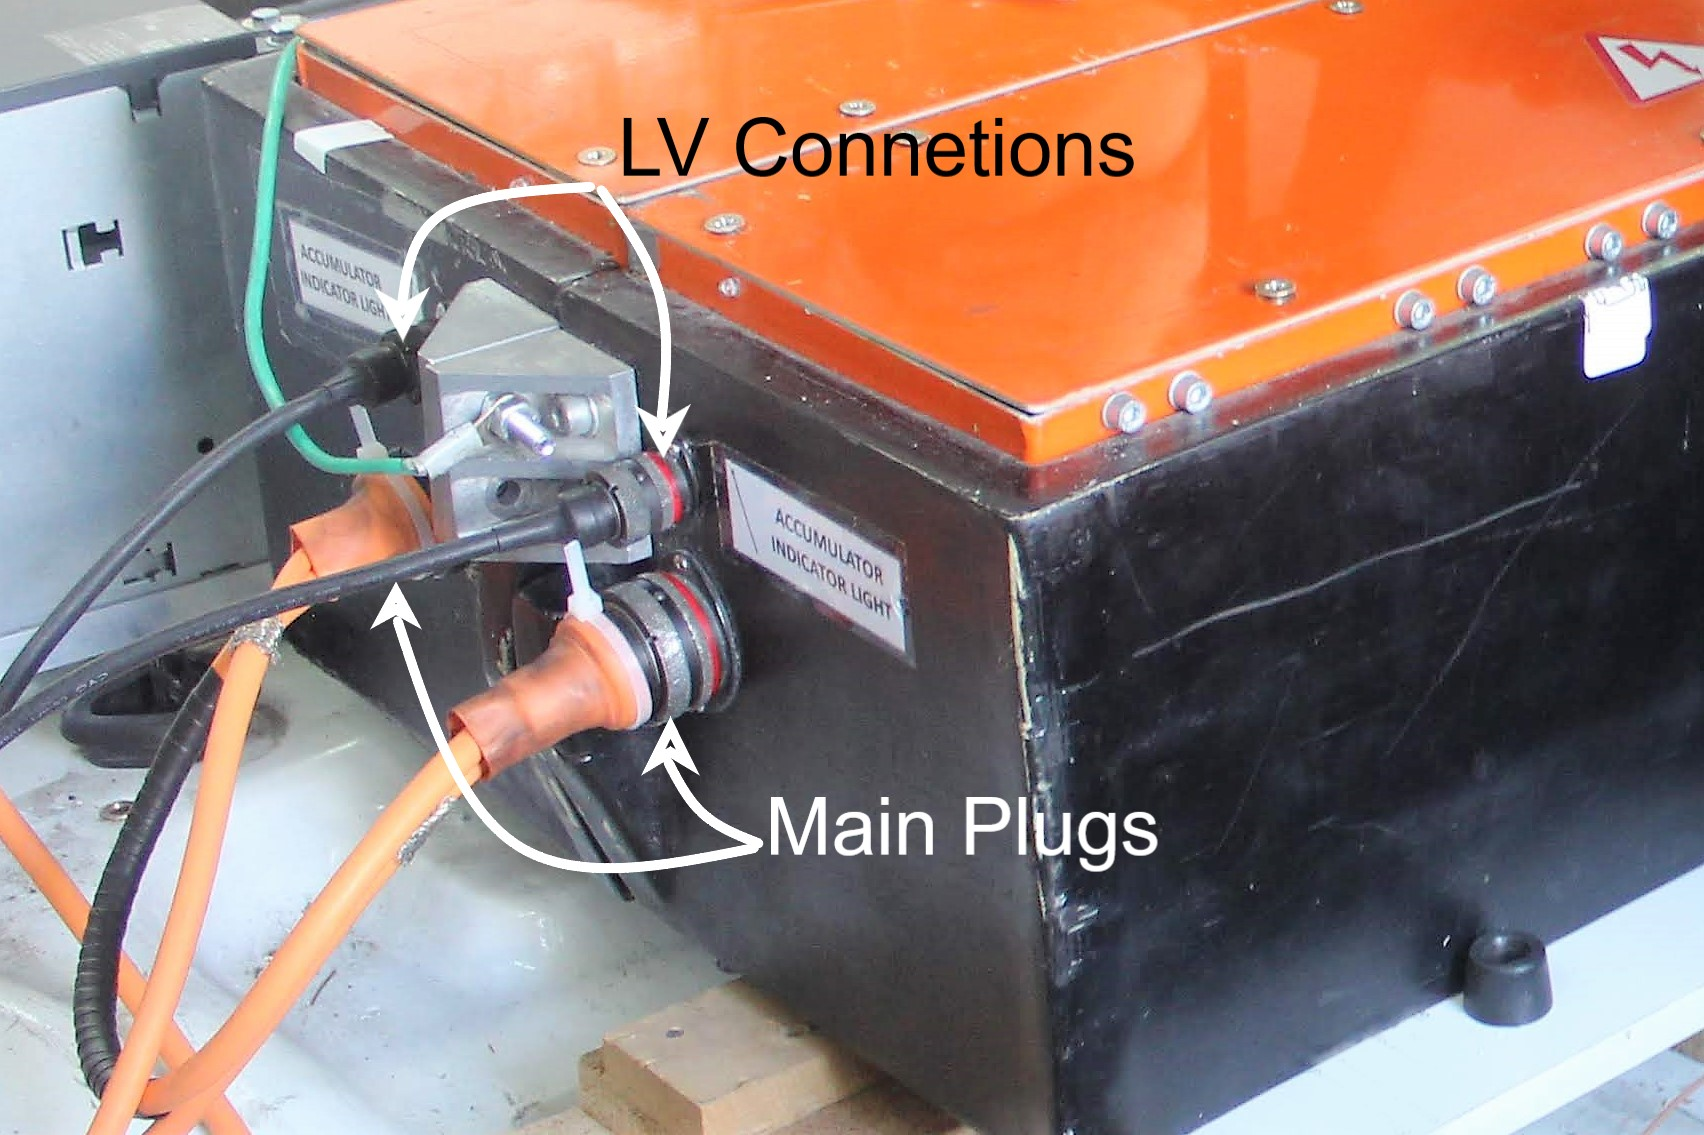
\includegraphics[width=0.7\linewidth]{figures/main_battery_connections}
	\caption{Main battery pack and connectors}
	\label{fig:battery_connections}
\end{figure}

\begin{table}[!hb]
	\centering
	\begin{tabular}{lc}
		\toprule
		\textbf{Parameter} & \textbf{Value}\\
		\midrule
		Maximum tractive system voltage & 600 V \\
		Nominal tractive system voltage & 532,8 V \\
		Control system voltage & 24 V \\
		Accumulator configuration & 144s1p \\
		Total accumulator capacity & 10 Ah\\
		\bottomrule
	\end{tabular}
	\caption[Battery pack specifications]{Battery pack specifications (source \cite{fst06})}
	\label{tab:battery_pack_specs}
\end{table}

\subsection{Connections}
The low voltage connectors contain 22 numbered pins listed in table \ref{tab:lv_connections} with respective description of them plus the expected connection. The expected connection is not the original intended connection signal since they were designed for use within \gls{FST} championships and have to oblige several protections like automatic cut power in case of water leakage detection inside specific compartments for instance. Majority of those rules, do not apply for our case. As so, all \gls{AIR} feeds are connected to 24V. Basically \gls{AIR} feeds act similar to a series of safety interrupters that must be active to provide high voltage but in this case is bypassed. Description of pins were provided by \gls{FST} members.

\begin{mdframed}[backgroundcolor=red!20, roundcorner=10pt, innertopmargin=5pt, innerbottommargin=5pt, skipabove=5pt]
	\Warning \, \textbf{The CAN connections are not internal terminated with the 120 $\Omega$ resistor.}
\end{mdframed}

\begin{table}
	\centering
	\begin{tabular}{cclcc}
		\toprule
		\textbf{Group} & \textbf{Pin Number} & \textbf{Description} & \textbf{Cable color} & \textbf{Value}\\
		\midrule
		% group supply
		\multirow{2}{*}{Supply}& 1 & GND     & yellow & GND	\\
		 & 2 & VCC\_A1 & white  & 24V \\
		 \midrule
		 & 3 & \multicolumn{3}{c}{Not used} \\
		 \midrule
		 % group AIR
		 \multirow{2}{*}{AIR} & 4 & AIR     & white  & 24V \\	
		 & 5 & AIR     & white  & 24V \\
		 % group AIR_supply
		 \midrule
		 \multirow{2}{*}{AIR Supply}& 6 & GND	    & yellow & GND \\
		 & 7 & VCC\_AIR  & white  & 24V \\
		 % group Fans
		 \midrule
		 Fans & 8 & GND	    & yellow & GND \\
		 (not used in this version) & 9 & VCC\_AIR  & white  & 24V \\
		 \midrule
		 \vspace{1pt}\\
		 \multicolumn{5}{c}{Pins 10 to 19 are not used}\\
		 \vspace{1pt}\\
		 \midrule
		 \multirow{2}{*}{CAN}& 20 & CAN\_L & Black & CAN Low \\
		 & 21 & CAN\_H  & Black  & CAN High \\
		 \midrule
		  & 22 & \multicolumn{3}{c}{Not used} \\
		\bottomrule
	\end{tabular}
	\caption{Main battery low voltage connections description}
	\label{tab:lv_connections}
\end{table}


\subsection{List of CAN messages}
The interface between user and main battery pack master controller consists in the following CAN messages:
\begin{description}
	\item[Queries list:] \
	\begin{description}
		\item[Reset] Demand reset. Performs a system reset.
		\item[TS ON OFF] Toggle tractive system on or off. This enables or disables the main supply of high \gls{DC} voltage.
		\item[Reset AMS error] Resets any error or warning related to \gls{AMS}. This can happen if:
		\begin{itemize}
			\item highest single cell voltage is above 4.1 V.
			\item lowest single cell voltage is bellow 3.2 V.
		\end{itemize}
		\item[Toggle verbose] Master boards enters verbose and fowards all messages received from slaves to outside.
		\item[Fake error] Executes turn off sequence and fakes \gls{AMS} fault. Not expected to be used.
		\item[Override mode] Overrides most \gls{AMS} faults. Not expected to be used. 
	\end{description}
	\item[Broadcast list] \
	\begin{description}
		\item[SOC] Report \gls{SoC} of battery pack.
		\item[Voltage] Report voltage level of battery pack.
		\item[Cell voltages] Report highest, average and lowest cell voltages.
		\item[Cell Temperatures] Report highest, average and lowest cell temperatures.
	\end{description}
	\item[Emergency] Report message with module issuing the emergency with respective error code.
\end{description}

Each message has the following typical structure presented in table \ref{tab:can_structure_main_battery}. To see the full list and respective CAN ID  values, check \href{https://docs.google.com/spreadsheets/d/125uncR7r-g646vKBvJf47TaTHI3FF9lcHkIi9cz6BJQ/edit?usp=sharing}{here} and the source code of CANInterface application (see next section)

\begin{table}[!hb]
	\centering
	\begin{tabular}{lc}
		\toprule
		\textbf{Field} & \textbf{Value}\\
		\midrule
		\multicolumn{2}{c}{\textbf{Queries messages}}\\
		\midrule
		CAN ID & CAN\_ID\_BMS\_CONTROL\_\\
		DLC & 4\\
		Data word 0 & Timestamp (lower 16bits)\\
		Data word 1 & command identifier requested\\
		\midrule
		\multicolumn{2}{c}{\textbf{Broadcast messages}}\\
		\midrule
		CAN ID & Message type dependent \\
		DLC & Message type dependent (from 4 to 8)\\
		Data word 0 & Timestamp (lower 16bits)\\
		Data word 1 & Message type dependent \\
		Data word 2 & Message type dependent \\
		Data word 3 & Message type dependent \\
		\midrule
		\multicolumn{2}{c}{\textbf{Emergency messages}}\\
		\midrule
		CAN ID & CAN\_ID\_BMS\_FAULT\\	
		DLC & 6\\	
		Data word 0 & Timestamp (lower 16bits)\\	
		Data word 1 & Issuing module id\\
		Data word 2 &Emergency code\\	
		\bottomrule
	\end{tabular}
	\caption{Typical CAN messages structure for main batteries pack}
	\label{tab:can_structure_main_battery}
\end{table}

\subsection{Enabling and disabling power}
Currently, for enabling the battery main battery power pack it is required an additional circuit sniffer. This is caused by the fact that during the programming and construction of the battery packs a mistake was made in the \gls{CAN} interface, where oscillator crystals used have a natural frequency of 15MHz, but the programming was made assuming it would be 16MHz. This causes an unreproducible CAN bit rate timing of $937.5\text{Kbps}$ when it was expected $1\text{Mbps}$. While the correction of this bug is simply done by reducing one time quantum for example in the propagation phase segment and reprogram all the 14 boards (two masters plus 12 slaves) inside the main battery pack. While the solution seems simple, in practice, this is considered a precision and risk task due to the construction and difficult of battery pack disassemble. The \gls{FST} have alerted for such risk and advised that should only be done if strictly necessary. For this reason the sniffer tool is used which was made using the exact same configuration as the internal circuit boards inside the main battery pack, causing it to be equivalent and enabling communication between them.
The connection to sniffer tool is done via USB port.

\begin{mdframed}[backgroundcolor=red!20, roundcorner=10pt, innertopmargin=5pt, innerbottommargin=5pt, skipabove=5pt]
	\Warning \, \textbf{When active, the main battery pack draws near 3A of current majority of them used in the activation of high voltage relays. The auxiliary pack must be able to support such need. Such power is temporary provided by two 12V lead acid batteries.}
\end{mdframed}

\begin{figure}[!hb]
	\centering
	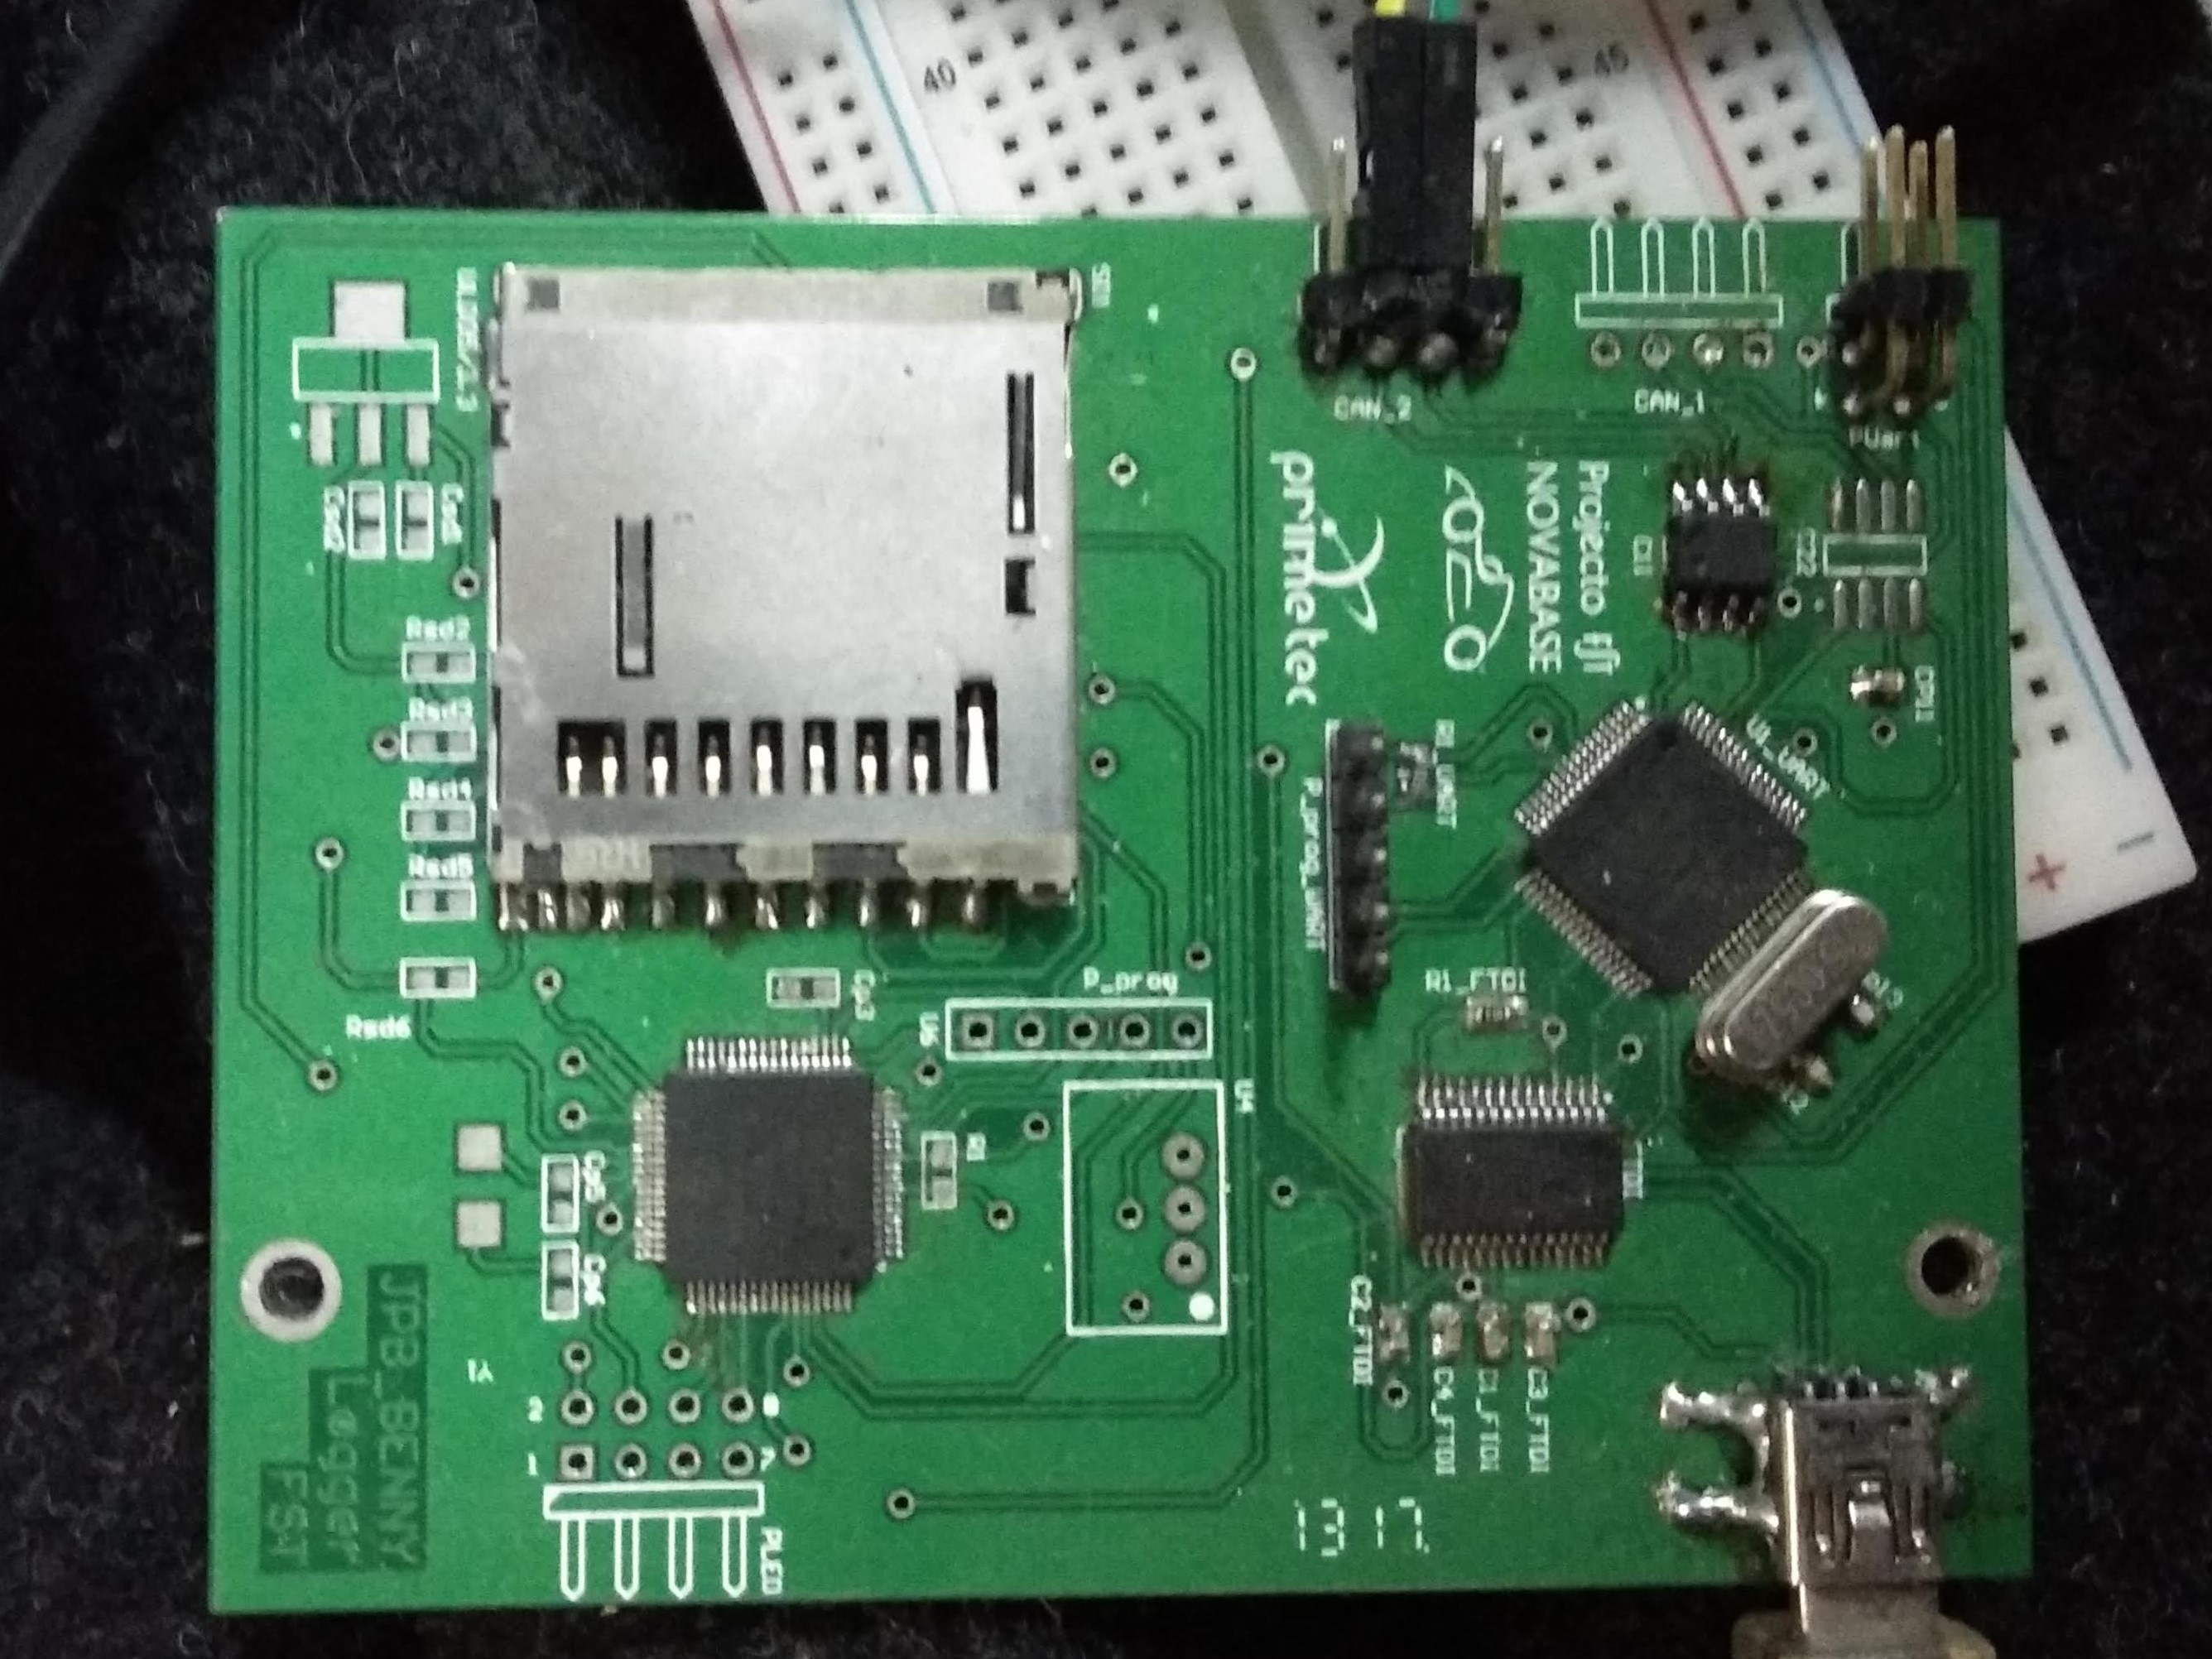
\includegraphics[width=0.5\linewidth]{figures/battery_pack_can_sniffer}
	\caption{Battery pack CAN sniffer}
	\label{fig:battery_can_sniffer}
\end{figure}

To enable power, it used the CANinterface application. It can be acquired \href{https://drive.google.com/drive/folders/14vwq4Xsy3RlByVp1BpFwrFQleFbBh3zu?usp=sharing}{here}. To compile, it is necessary to use the Qt libraries. Current makefile is for Linux, but since Qt is known for being cross-platform, it should work in other OS systems. Install requirements using: 

\begin{lstlisting}[frame=none,language=bash,backgroundcolor=\color{gray!15},numbers=none, basicstyle=\ttfamily]
sudo apt install qt5-default qt5-qmake libqt5serialport5-dev
\end{lstlisting}

After download it, simply use \console{make} to compile program. By default it will be compiled into release folder inside the extracted root folder. Change to that directory and run it using \console{./CANinterface}. Figure \ref{fig:interface_opening} show the expected GUI. First it is needed to place the correct USB port. \textbf{The baudrate is 460800.} If battery pack is correctly powered up and \gls{CAN} line is correctly connected, it should start showing the messages received on console tab. 

\begin{figure}
	\centering
	\subcaptionbox{Opening screen of interface}{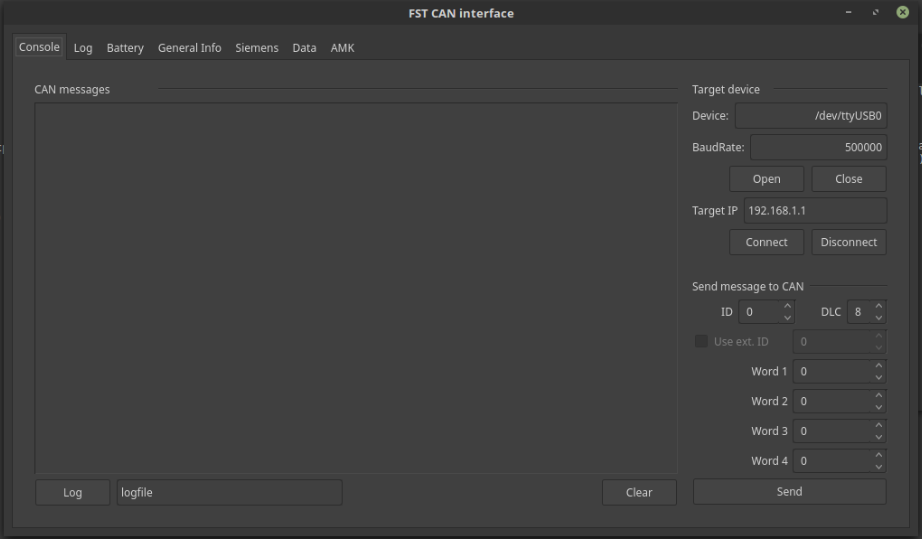
\includegraphics[width=0.7\linewidth]{figures/interface_01}}\\
	\subcaptionbox{Baudrate settings}{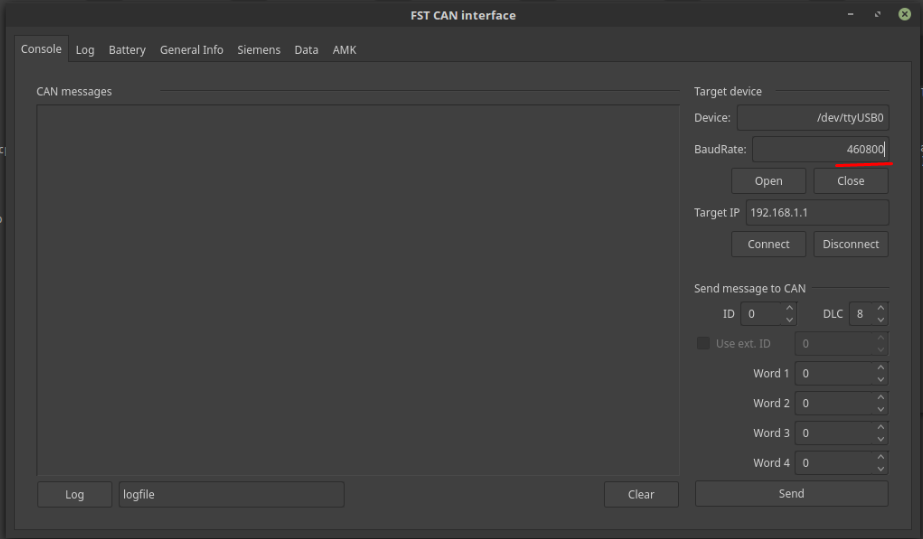
\includegraphics[width=0.7\linewidth]{figures/interface_02}}\\
	\subcaptionbox{Sucessful connection}{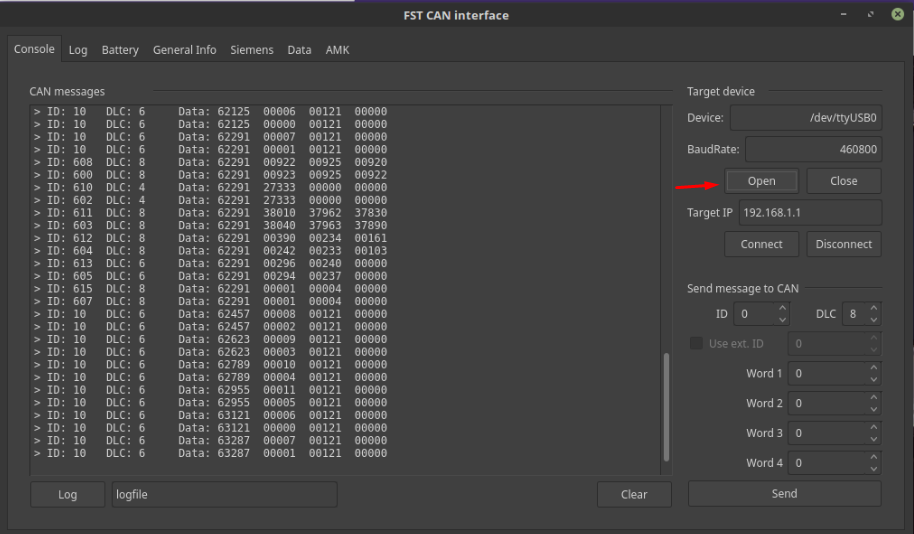
\includegraphics[width=0.7\linewidth]{figures/interface_03}}
	\caption{CANinterface GUI - opening}
	\label{fig:interface_opening}
\end{figure}

To enable power, switch to battery tab. In this tab it show the status of main battery pack. From this tab is important to retain information especially related to minimum cell voltage. If this value are near to 3.2V, it is time to recharge the pack, since it is the recommended minimum value for this type of cells used inside main battery pack.
Check if the \gls{AIR} feedback is green. The \gls{AIR} if not, main battery pack will not be able to engage. Check the connections as shown in table \ref{tab:lv_connections}. 
Before enabling power, it is important to check if the pre-charge circuit is working ok.
For that, use the installed multimeter to measure the \gls{DC} voltage applied to Siemens frequency inverter. When the power is enabled, check if the \gls{DC} voltage start to grow. The pre-charge circuit is bypassed after five seconds. 
\begin{mdframed}[backgroundcolor=red!20, roundcorner=10pt, innertopmargin=5pt, innerbottommargin=5pt, skipabove=5pt]
	\Warning \, \textbf{If the voltage is not increasing within the five seconds, user must use the emergency button to disable power source for main battery or circuits after may be irreversible damaged!}
\end{mdframed}

As so, before enabling power, make sure multimeter is set and prepare to press the emergency button if required. After this, press the \console{TS on/off} button. The TS on feedback will be green. User will heard the two relays engaging. Look at multimeter immediately after this! If it shows voltage value rising all is ok and after five seconds the bypass relay is engaged. 
\begin{mdframed}[backgroundcolor=red!20, roundcorner=10pt, innertopmargin=5pt, innerbottommargin=5pt, skipabove=5pt]
	\Warning \, \textbf{Power is now on! Serious risk of death if user touch the high voltage line}
\end{mdframed}
	
\begin{figure}
	\centering
	\subcaptionbox{Battery tab}{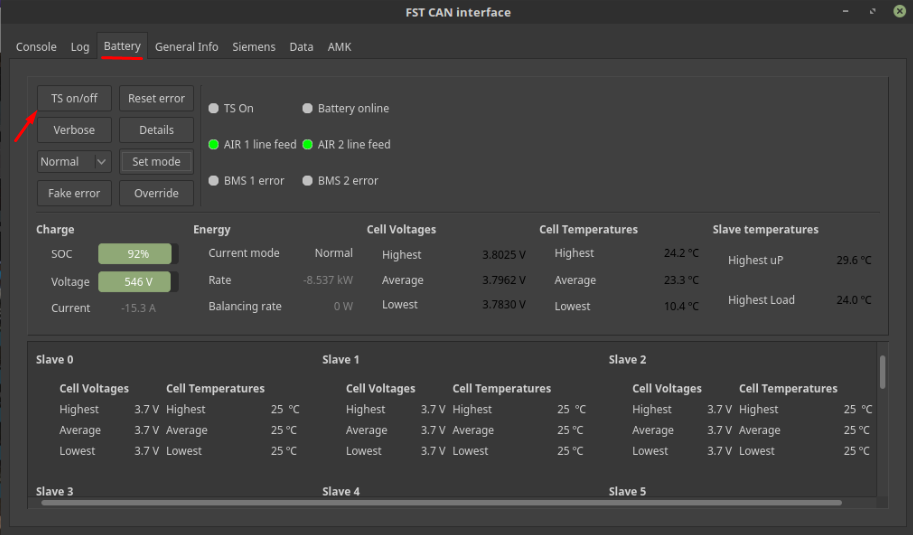
\includegraphics[width=0.7\linewidth]{figures/interface_04}}\\
	\subcaptionbox{Enabling power}{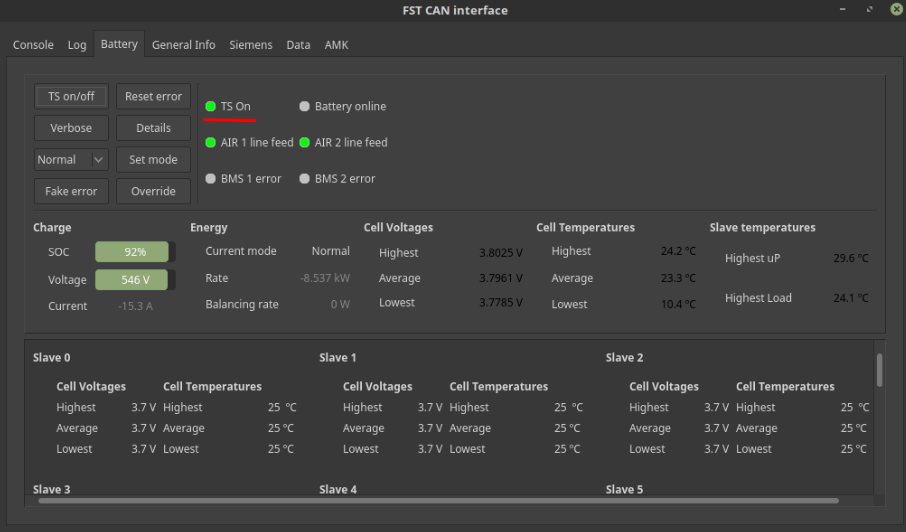
\includegraphics[width=0.7\linewidth]{figures/interface_05}}
	\caption{CANinterface GUI - enabling power}
\end{figure}

For disabling power, user can simply press the emergency button or use the interface and press again the \console{TS on/off} button.
\begin{mdframed}[backgroundcolor=red!20, roundcorner=10pt, innertopmargin=5pt, innerbottommargin=5pt, skipabove=5pt]
	\Warning \, \textbf{Even after disabling power the voltage drop takes time, check in the multimeter to make sure to check multimeter in order to see if it has reached 0V before perform any interaction with the high voltage line.}
\end{mdframed}

\section{Auxiliary battery pack}
As said before, power for main battery packs is drawn from two 12V lead acid batteries connected in series. It must meet the requirements of near 3A when main voltage is applied to Siemens inverter.

Another pack of batteries is currently used to provide power for \gls{Rpi}, \gls{GNSS} receivers, \gls{AHRS} sensor and \gls{EPOS} device. The battery type are \gls{LiPo} produced by \href{kokam.com}{KoKam} model SLPB75106100 \cite{lipo_kokam}. Those packs currently do not have any \gls{BMS}, although is currently in study and preliminary design a structure for low voltage supply based on a \gls{BMS} and \gls{DC}/\gls{DC} converters for the several voltage levels needed.
 
All negative poles must be shared together from all batteries packs to avoid noise. That is currently made using the chassis as ground plane as shown in figure \ref{fig:common_ground}.

\begin{figure}[]
	\centering
	\subcaptionbox{Back connection}{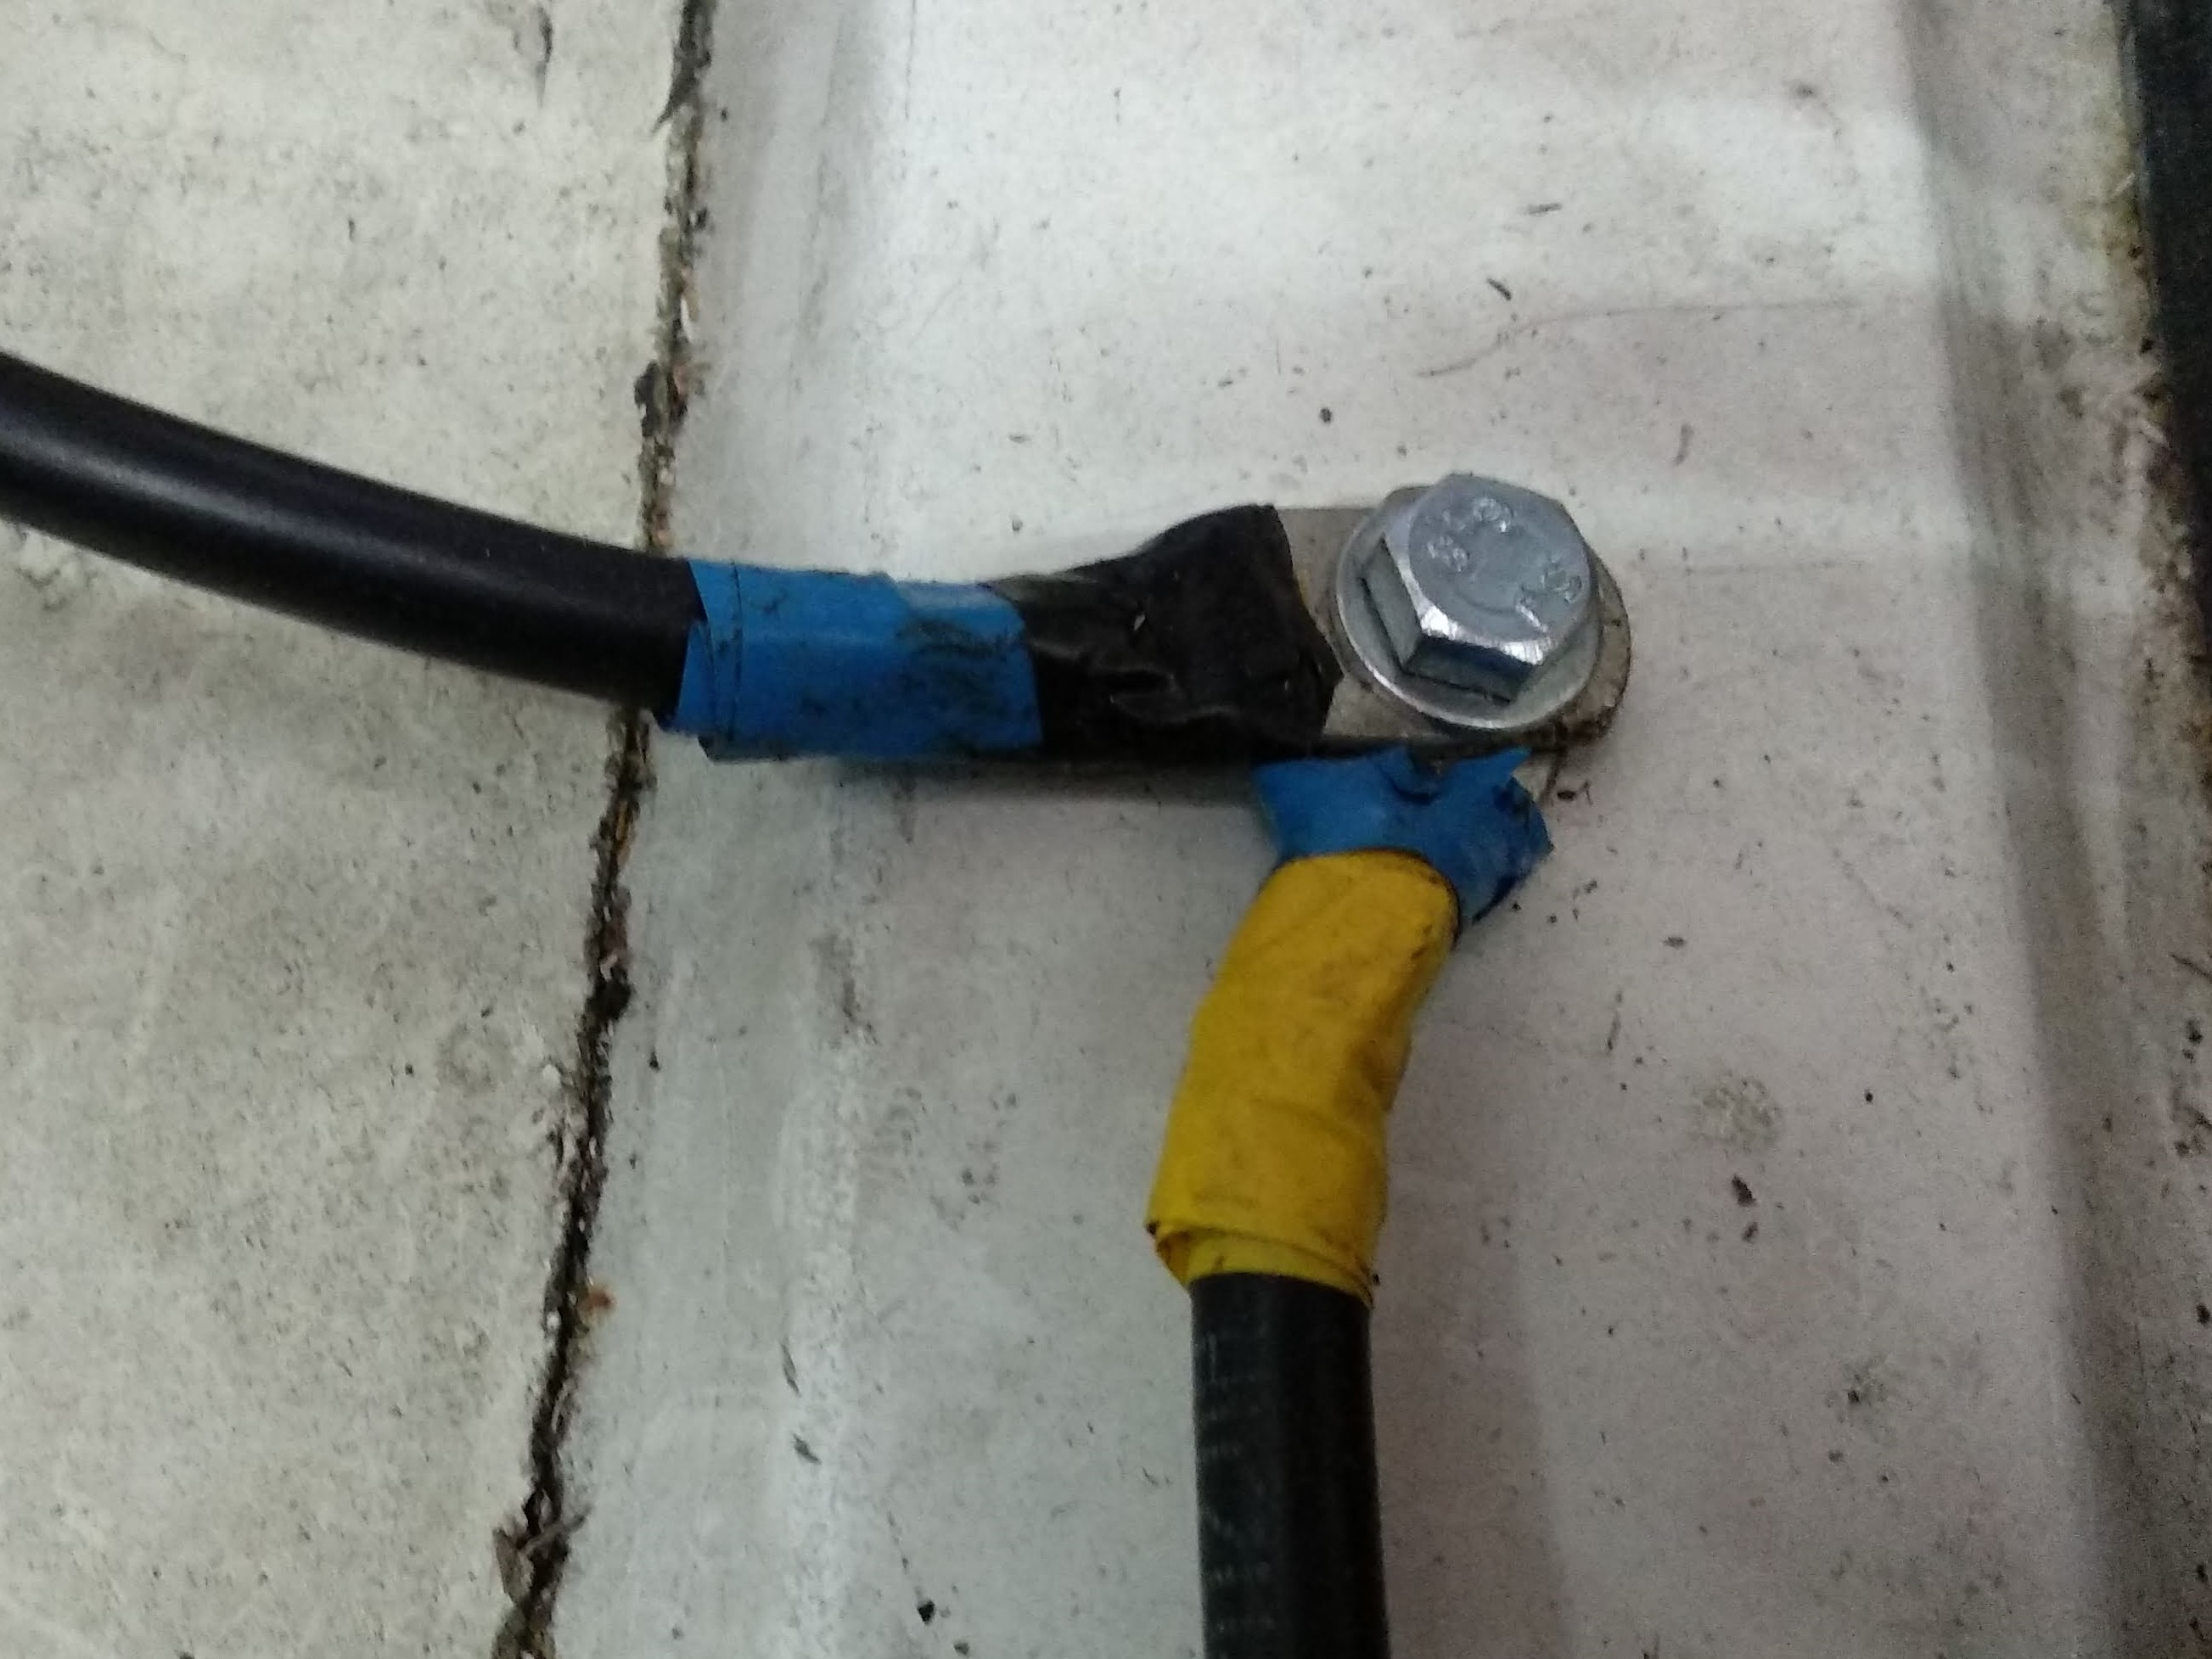
\includegraphics[width=0.45\linewidth]{figures/common_ground_1}}
	\subcaptionbox{Front connection}{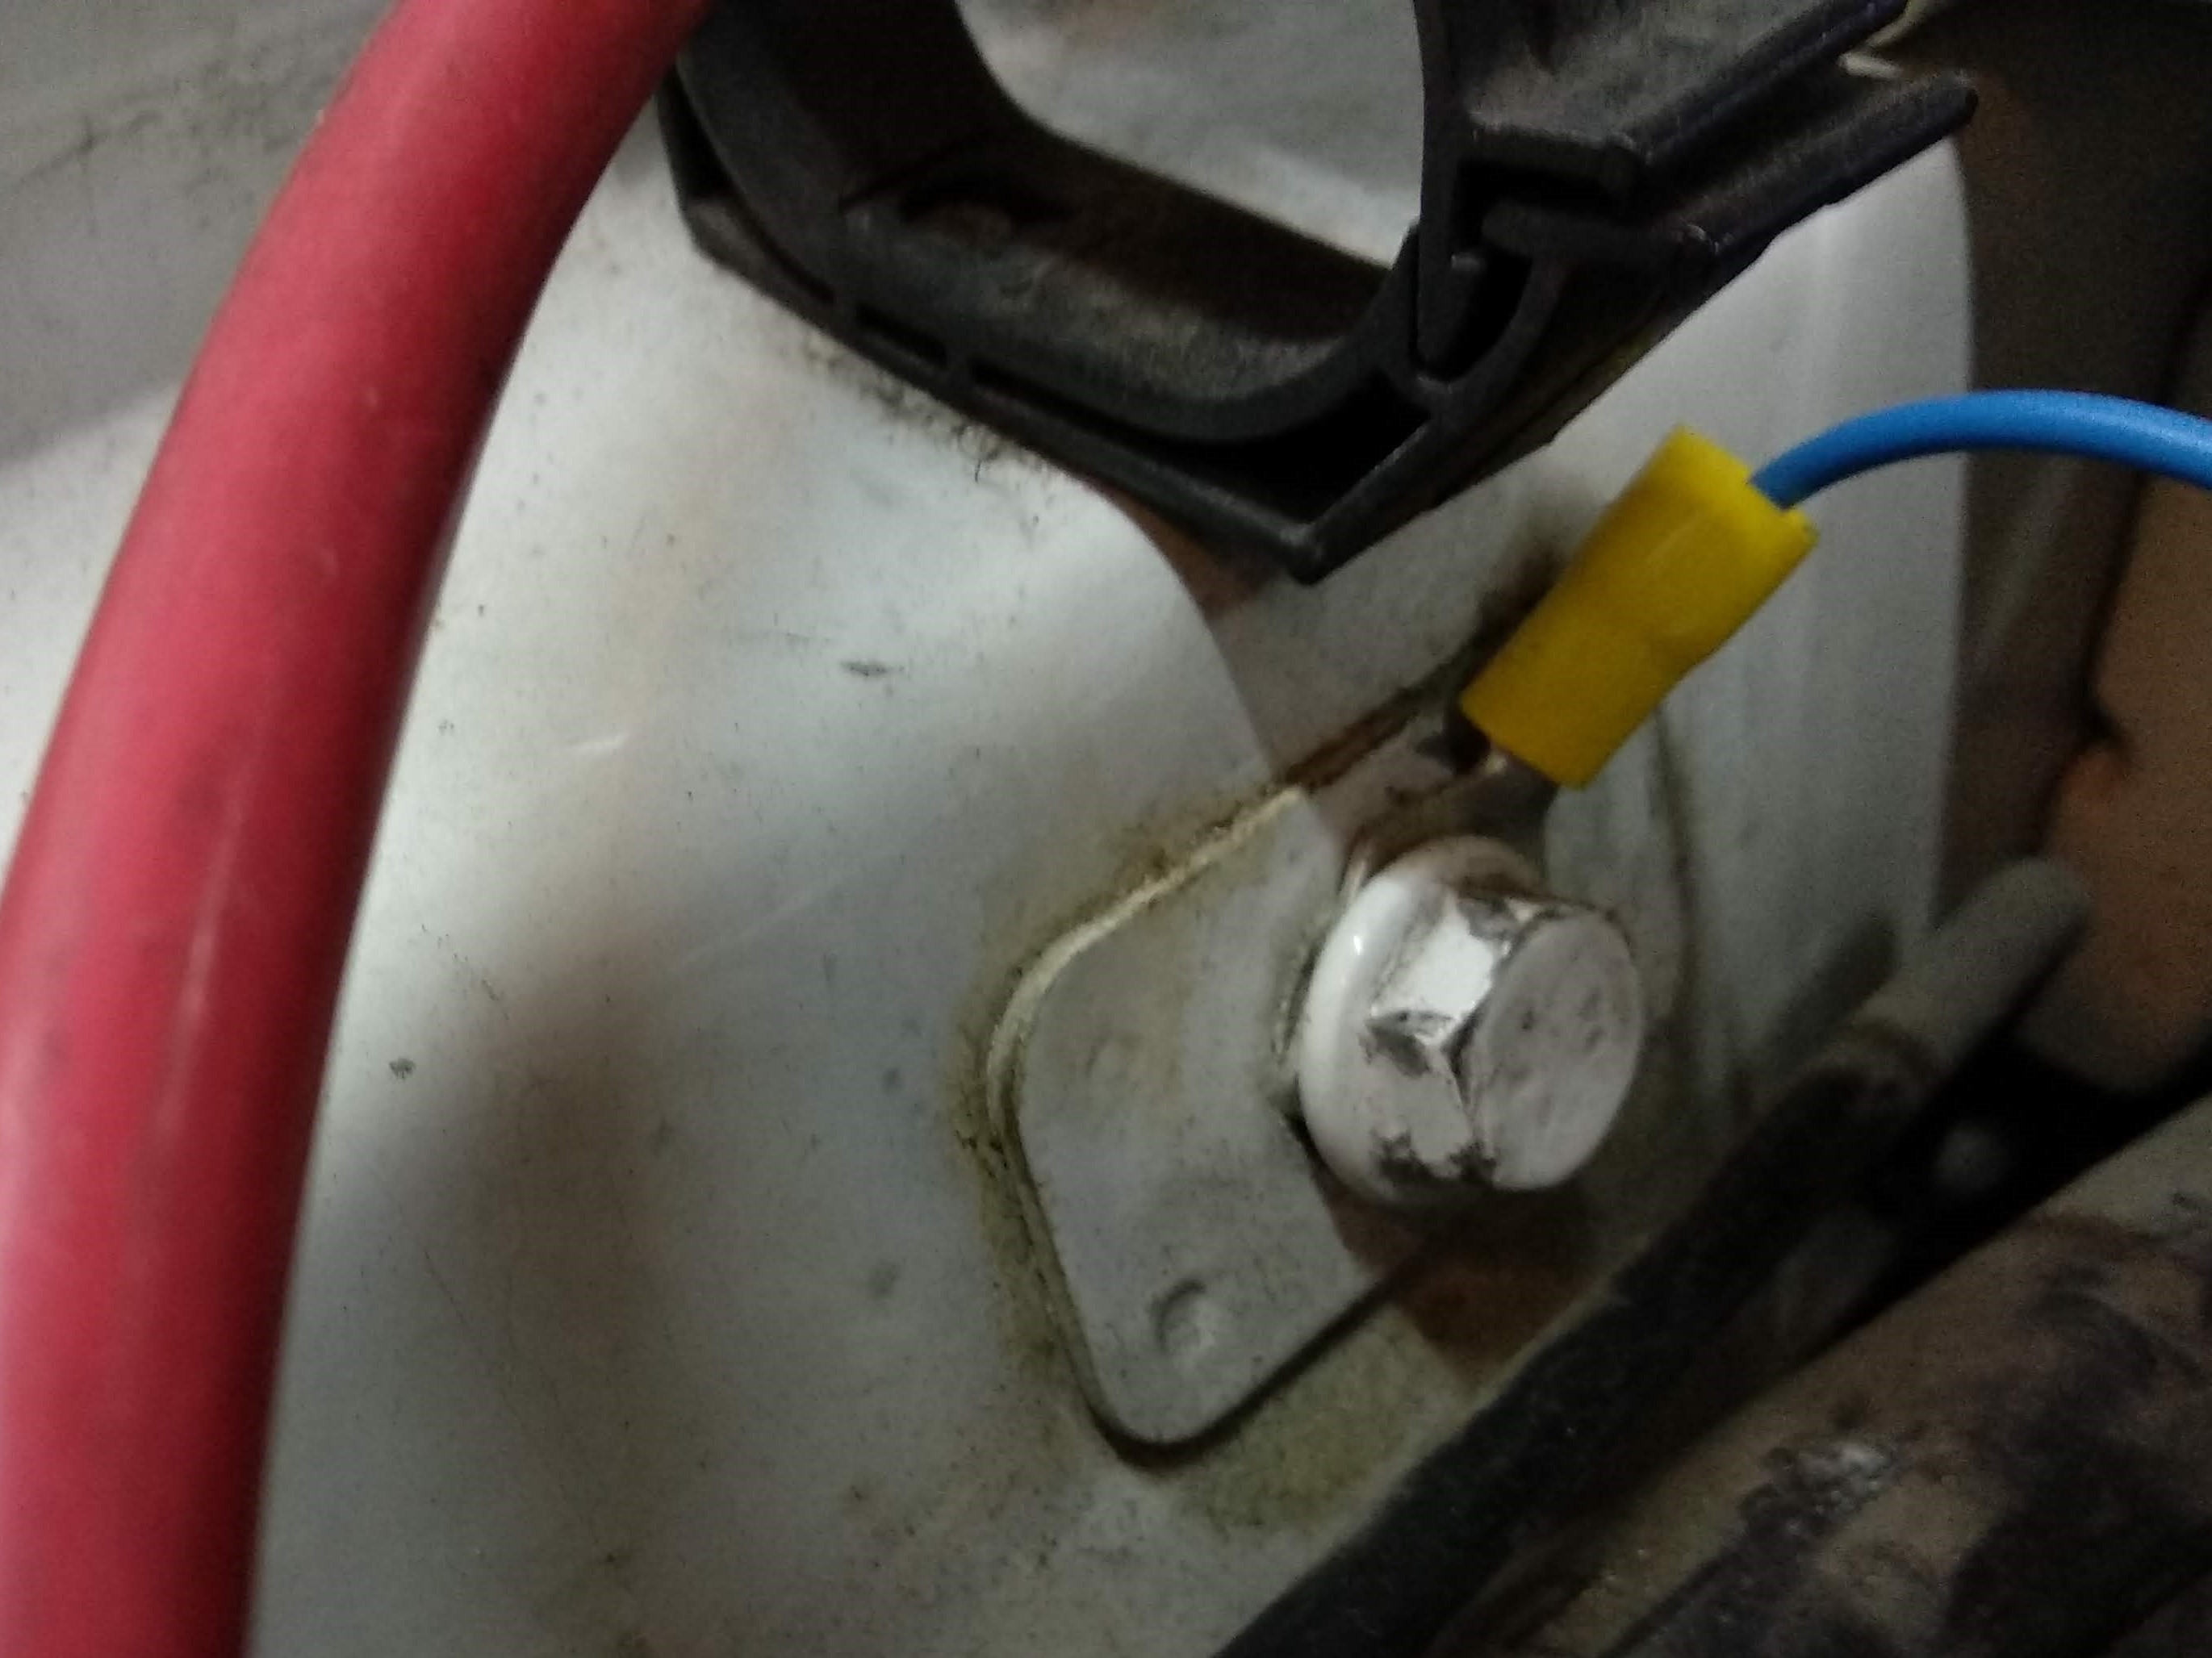
\includegraphics[width=0.45\linewidth]{figures/common_ground_2}}
	\caption{Common ground connections example}
	\label{fig:common_ground}
\end{figure}
